% !TEX encoding = UTF-8 Unicode
\documentclass{beamer}
\usetheme{Szeged}

\usepackage{color}
\usepackage{url}
\usepackage[utf8]{inputenc}
\usepackage{graphicx}

\usepackage[english, serbian]{babel}

%\usepackage[unicode]{hyperref}
\usepackage{amsmath}
\usepackage{amsthm}
\usepackage{amssymb}
\hypersetup{colorlinks,citecolor=green,filecolor=green,linkcolor=blue,urlcolor=blue}
\usepackage[title]{appendix}
\usepackage{float}
\usepackage[graphicx]{realboxes}
\usepackage{chngcntr}
\counterwithin{figure}{section}
\usepackage{listings}
\usepackage{textcomp}
\usepackage{xcolor}
\usepackage{adjustbox}
\lstset {
    language=Python,
    frame=none,
    %xleftmargin=-.25in,
    %xrightmargin=.25in
    framesep=10pt,
    tabsize=4,
    showstringspaces=false,
    upquote=true,
    commentstyle=\color{gray},
    keywordstyle=\color{orange},
    stringstyle=\color{red},
    basicstyle=\scriptsize\ttfamily,
    emph={int,char,double,float,unsigned,void,bool},
    emphstyle={\color{blue}},
    escapechar=\&,
    classoffset=1,
    morekeywords={>,<,.,;,,,-,!,=,~},
    keywordstyle=\color{weborange},
    classoffset=0,
    breaklines=true
}

\usepackage[font=scriptsize,labelfont=bf]{caption}


\title{Automatsko generisanje plejlisti}

\author{\href{mailto:mi14031@matf.bg.ac.rs}{Ivan Ristović}, \href{mailto:mi14042@matf.bg.ac.rs}{Milana Kovačević}
}
\date{septembar 2018.}


\begin{document}
\begin{frame}
    \titlepage
\end{frame}

\begin{frame}{Zadatak}
    \begin{itemize}
        \item Na osnovu skupa podataka o raznovrsnim pesmama generisati plejliste
        \item Svaka generisana plejlista mora sadrzati ``sli\v{c}ne'' pesme (dozvoljene su male varijacije \v{z}anra, ja\v{c}ine itd.)
    \end{itemize}
\end{frame}

\begin{frame}{Skup podataka}
    \begin{itemize}
        \item Spotify
        \item R biblioteke za generisanje CSV fajlova
    \end{itemize}
\end{frame}

\begin{frame}{Kori\v{s}ceni modeli}
    \begin{itemize}
        \item Multinomijalna logisti\v{c}ka regresija
        \item SVM
        \begin{itemize}
            \item Linearni SVM
            \item Kernelizovani SVM
        \end{itemize}
        \item KNN
        \item Neuronske mre\v{z}e
    \end{itemize}
\end{frame}

\begin{frame}[fragile]{Multinomijalna logisti\v{c}ka regresija}
    \begin{figure}[!h]
    \centering
    \begin{tabular}{ | c | c | c | c | c |}
        \hline
        Skup & Broj instanci & Preciznost & Odziv & F1 mera \\
        \hline
        Trening & 14457 & 0.328215 & 0.328215 & 0.294002 \\
        Test & 6196 & 0.304874 & 0.304874 & 0.272252 \\
        \hline
    \end{tabular}
    \end{figure}
\end{frame}

\begin{frame}[fragile]{Linearni SVM}
    \begin{figure}[!h]
    \centering
    \begin{tabular}{ | c | c | c | c | c |}
        \hline
        Skup & Broj instanci & Preciznost & Odziv & F1 mera \\
        \hline
        Trening & 14457 & 0.316456 & 0.316456 & 0.268594 \\
        Test & 6196 & 0.308263 & 0.308263 & 0.260433 \\
        \hline
    \end{tabular}
    \end{figure}
\end{frame}

\begin{frame}[fragile]{Kernelizovani SVM}
    \begin{figure}[!h]
    \centering
    \begin{tabular}{ | c | c | c | c | c |}
        \hline
        Skup & Broj instanci & Preciznost & R2 skor & F1 mera \\
        \hline
        Trening & 14457 & ? & ? & ? \\
        Test & 6196 & ? & ? & ? \\
        \hline
    \end{tabular}
    \end{figure}
\end{frame}

\begin{frame}[fragile]{KNN}
    \begin{figure}[!h]
    \centering
    \begin{tabular}{ | c | c | c | c | c |}
        \hline
        Skup & Broj instanci & Preciznost & Odziv & F1 mera \\
        \hline
        Trening & 14457 & 0.363699 & 0.363699 & 0.316085 \\
        Test & 6196 & 0.233538 & 0.233538 & 0.202797 \\
        \hline
    \end{tabular}
    \end{figure}
\end{frame}

\begin{frame}[fragile]{Neuronske mre\v{z}e}
    \begin{figure}[!h]
    \centering
    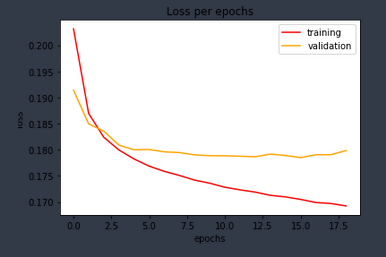
\includegraphics[scale=0.9]{loss.PNG}
    \end{figure}
\end{frame}

\begin{frame}[fragile]{Neuronske mre\v{z}e}
    \begin{figure}[!h]
    \centering
    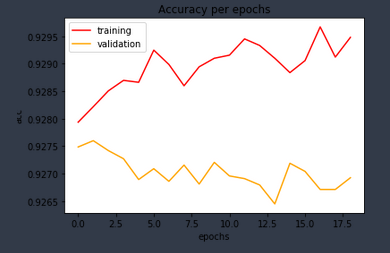
\includegraphics[scale=0.9]{acc.PNG}
    \end{figure}
\end{frame}

\begin{frame}{Pitanja}
    \centering
    ???
\end{frame}

\begin{frame}
    \centering
    Hvala na pa\v{z}nji!
\end{frame}

\end{document}
